% TRACE submission manuscript adapted for Intelligent Systems with Applications (Elsevier)
% Revision: decision-oriented evaluation, RSSM interpretation, explicit reproducibility caveats
% Source: condensed JBI version; numerical results preserved
\documentclass[preprint,12pt]{elsarticle}

\usepackage{orcidlink}
\usepackage{amsmath,amssymb}
\usepackage{booktabs}
\usepackage{graphicx}
\usepackage{tabularx}
\usepackage{array}
\usepackage{xcolor}
\usepackage{hyperref}
\usepackage{enumitem}
\usepackage{lineno}
\usepackage{subcaption}
\usepackage{tikz}
\usetikzlibrary{arrows.meta,positioning,fit}

\journal{Intelligent Systems with Applications}

\begin{document}
\setlength{\emergencystretch}{2em}
\begin{frontmatter}

\title{TRACE: Multi-Criteria Evaluation and Model Selection for Reliable Clinical Time-Series Simulation}

\author[aff1]{Nesma Settouti\corref{cor1}\orcidlink{0000-0003-0460-9713}}
\ead{nesma.settouti@isen-ouest.yncrea.fr}
\author[aff2]{Souaad Hamza-Cherif}
\author[aff3]{Mohammed El Amine Bechar}
\cortext[cor1]{Corresponding author}
\address[aff1]{LabISEN, LSL, ISEN Ouest, Caen, France}
\address[aff2]{Biomedical Engineering Laboratory, Tlemcen University, Tlemcen, Algeria}
\address[aff3]{LabISEN, LSL, ISEN Ouest, Brest, France}

\begin{abstract}

\textbf{Objective:}
Selecting intelligent time-series models using one-step prediction alone may be inadequate when the systems are deployed for recursive simulation. We investigated whether model preference remains stable when adequacy is defined by predictive fit, recursive state fidelity, temporal-change accuracy, temporal variability, uncertainty reliability, or robustness to heterogeneous observation density, and whether these selection patterns persist across hospital systems.

\textbf{Methods:}
We present TRACE, a protocol-defined multi-criteria evaluation framework for comparing intelligent time-series models according to deployment-relevant behavior. Linear autoregression, gated recurrent unit (GRU), Transformer, and recurrent state-space model (RSSM) architectures were trained with five fixed seeds on Set A of the PhysioNet/Computing in Cardiology Challenge 2019. Internal evaluation used a locked patient-disjoint Set A test cohort with 4-, 12-, 24-, and 48-h recursive mean rollouts and hierarchical paired bootstrap confidence intervals. Predictive fit, recursive state fidelity, temporal-change error, preservation of temporal variability, conditional predictive-interval reliability, and observation-density sensitivity were evaluated separately. After the internal analysis and interpretation rules were finalized, the same checkpoints, preprocessing, and evaluation definitions were applied without retraining or recalibration to held-out Set B from a second hospital system.

\textbf{Results:}
No criterion-independent model winner emerged. Transformer achieved the best validation NLL ($0.8394 \pm 0.0020$), the lowest internal one-step normalized MacroMAE (0.4076), and the most reliable conditional predictive intervals. At 48 h, Transformer and RSSM were statistically unresolved for recursive state fidelity (paired difference 0.0036, 95\% CI $[-0.0424, 0.0622]$). RSSM nevertheless achieved significantly lower DynamicMAE than Transformer (difference 0.00372, 95\% CI $[0.00093, 0.00650]$), while exhibiting stronger temporal variance contraction and poorer interval coverage. Relative model preference also changed across observation-density strata. On held-out Set B, the same multi-axis pattern persisted: predictive fit and interval reliability favored Transformer, temporal-change error favored RSSM, recursive state fidelity remained unresolved between them, and density-dependent selection persisted.

\textbf{Conclusion:}
Predictive fit, recursive state fidelity, temporal-change error, temporal variability, uncertainty reliability, and observation regime provide complementary rather than interchangeable evidence. Clinical trajectory models should therefore be evaluated and selected according to the properties required by their intended use rather than by a single predictive criterion.

\end{abstract}

\begin{keyword}
intelligent systems \sep
multi-criteria model evaluation \sep
clinical time series \sep
recursive forecasting \sep
model selection \sep
reliability assessment
\end{keyword}

\end{frontmatter}
\linenumbers

% =========================================================
\section{Introduction}
% =========================================================

Clinical time-series models are usually selected as predictors: given recent observations, they are judged by how accurately they predict the next state or a fixed future window. This is appropriate for local forecasting, but it is not sufficient when a model is expected to generate trajectories recursively. Once predictions are fed back as inputs, local errors become part of the future conditioning history and may produce drift, excessive smoothing, variance inflation, or unreliable uncertainty.

The distinction is especially important in critical care, where physiological trajectories are multivariate, irregularly observed, and heterogeneous in measurement density. Frequently recorded vital signs and sparsely measured laboratory variables may favor different inductive biases. A single global predictive score can therefore obscure properties that matter for longitudinal use: whether generated states remain close to observations, whether temporal changes and variability are preserved, whether predictive intervals remain credible, and whether conclusions depend on observation regime.

Clinical forecasting methods such as GRU-D, Temporal Fusion Transformers, t-PatchGNN, and recent irregular-time-series architectures are mainly evaluated using likelihood, pointwise error, discrimination, or fixed-window forecasting accuracy \cite{che2018grud,lim2021tft,zhang2024tpatchgnn,liu2026mtfpdg}. Medical world-model studies increasingly add longer-horizon trajectories, distributional properties, treatment-conditioned evolution, and closed-loop behavior \cite{makarov2025dtgpt,yang2025mewm,mu2026ehrworld,wang2026chronomedicalworld,wu2026sepsisagent}. These developments broaden evaluation, but they do not directly answer a model-selection question: \emph{would the same candidate model be selected when adequacy is defined by different properties required for longitudinal use?}

TRACE addresses this question as an evaluation problem rather than proposing a new forecasting architecture. Four deliberately contrasting model families---Linear AR, GRU, Transformer, and RSSM---serve as probes of the selection process. We ask whether rankings remain stable across predictive fit, recursive state fidelity, temporal-change accuracy, temporal variability, probabilistic reliability, and observation-density strata, and whether apparent reversals are statistically supported rather than numerical fluctuations.

The study uses the PhysioNet/Computing in Cardiology Challenge 2019 data \cite{reyna2020sepsis}. Set A supports training, validation, and a locked patient-disjoint internal evaluation. Only after the internal analysis and interpretation rules were finalized were the same checkpoints and definitions applied to held-out Set B from a second hospital system. Set B therefore tests whether the multi-axis selection pattern transports, not whether a new model should be selected.

The contributions are threefold. First, TRACE formulates trajectory evaluation as a \emph{model-selection consistency} problem: a model favored under one-step likelihood must not be presumed preferable for a different deployment requirement. Second, it specifies an auditable, requirement-to-evidence mapping across recursive state error, temporal-change error, temporal variability, conditional interval reliability, and observation-density sensitivity. The mapping does not introduce a new performance metric or assume that its axes can be combined into a universally valid scalar score. Paired hierarchical inference distinguishes supported preferences from numerical ordering alone. Third, TRACE tests whether these axis-specific conclusions persist under a frozen evaluation protocol in a second hospital system, while restricting its claims to observational dynamics rather than causal or counterfactual validity.

The remainder of the paper reviews the most relevant forecasting, world-model, and credibility literature; defines the TRACE protocol; reports internal and held-out results; and discusses implications for longitudinal clinical simulation.

% =========================================================
\section{Related work}
\label{sec:related}
% =========================================================

\subsection{Irregular clinical forecasting and multi-step prediction}

Missingness-aware recurrent models such as GRU-D and BRITS established that observation masks and elapsed time can be predictive in clinical data \cite{che2018grud,cao2018brits}. Continuous-time approaches, including GRU-ODE-Bayes, Latent ODEs, and neural controlled differential equations, model irregular trajectories more directly \cite{debrouwer2019gruodebayes,rubanova2019latentode,kidger2020neuralcde}. Attention-based and graph-based alternatives such as Multi-Time Attention Networks, Temporal Fusion Transformers, and t-PatchGNN further exploit temporal and cross-variable structure \cite{shukla2021mtan,lim2021tft,zhang2024tpatchgnn}. Their evaluation is nevertheless dominated by predictive error, likelihood, discrimination, or predefined forecasting windows.

Recursive forecasting raises a different issue because previous predictions become future inputs, allowing errors to accumulate \cite{bentaieb2012multistep}. DeepAR similarly generates future trajectories sequentially from conditional predictive distributions \cite{salinas2020deepar}. In ICU forecasting, DRIFT combines direct multi-horizon prediction with a constrained recursive, intervention-conditioned correction mechanism \cite{liu2026drift}. TRACE does not compare direct and recursive forecasting strategies; it asks whether the criterion used to judge candidate models changes the selection decision.

Probabilistic forecasting adds another distinction. Proper scoring rules assess predictive distributions, whereas calibration and sharpness describe complementary aspects of reliability \cite{gneiting2007scoring,gneiting2007calibration}. Nominal predictive intervals may be miscalibrated even when a model achieves favorable scoring-rule values \cite{gneiting2007calibration}. Consequently, one-step likelihood, recursive point error, temporal behavior, and interval coverage should not be assumed to measure the same property.

\subsection{PhysioNet 2019, medical world models, and fit-for-purpose credibility}

PhysioNet 2019 was introduced for early sepsis prediction \cite{reyna2020sepsis}, and much subsequent work has focused on classification or missingness-aware prediction \cite{singh2021missingness,kim2024temporalprior}. Liu et al. used the dataset for 24-to-24-h multivariate forecasting with point-error metrics and missingness robustness \cite{liu2026mtfpdg}. TRACE instead uses it to test recursive model-selection consistency (Table~\ref{tab:physionet_positioning}).

\begin{table}[ht]
\centering
\caption{Positioning relative to representative work using PhysioNet 2019.}
\label{tab:physionet_positioning}
\small
\begin{tabularx}{\textwidth}{p{2.3cm}p{2.8cm}p{2.8cm}X}
\toprule
Study & Primary task & Main evaluation & Distinction from TRACE \\
\midrule
Reyna et al. \cite{reyna2020sepsis} & Early sepsis prediction & Utility/discrimination & Endpoint classification; no recursive state simulation \\
Singh et al. \cite{singh2021missingness} & Missingness-aware prediction & Predictive performance/robustness & Missingness as signal; no trajectory-fidelity analysis \\
Kim \& Lee \cite{kim2024temporalprior} & Temporal-prior EHR prediction & Classification performance & Predictive architecture comparison \\
Liu et al. \cite{liu2026mtfpdg} & 24$\rightarrow$24 h forecasting & MSE, MAE, MRE, RMSE, MAPE & Direct fixed-window forecast \\
TRACE & Recursive trajectory evaluation & Fit, rollout, dynamics, reliability, density & Tests criterion-dependent selection and transportability \\
\bottomrule
\end{tabularx}
\end{table}

The world-model literature makes repeated transition quality central to model usefulness \cite{ha2018worldmodels,hafner2019planet}. Medical extensions now evaluate longitudinal trajectories, treatment-conditioned evolution, or closed-loop simulation \cite{makarov2025dtgpt,yang2025mewm,mu2026ehrworld,wang2026chronomedicalworld,wu2026sepsisagent}, and recent synthesis emphasizes trajectory-level evaluation and calibrated uncertainty \cite{liu2026medicalworldmodels}. Digital-twin credibility frameworks likewise argue that verification, validation, and uncertainty quantification should be fit for purpose and strengthen with the claim being made \cite{nasem2024digitaltwins,tudor2025hdt,sel2025vvuq,vallee2026trustworthy}. TRACE adopts this fit-for-purpose logic but deliberately stops at observational dynamics: PhysioNet 2019 does not support validation of counterfactual treatment response.

% =========================================================
\section{Materials and methods}
% =========================================================

\subsection{Study design and data}

TRACE used a two-stage protocol. Set A of PhysioNet 2019 was used for model fitting, validation-based checkpoint selection, and a locked patient-disjoint internal test; Set B was reserved for hospital-system transportability. Model families, preprocessing, rollout horizons, evaluation axes, observation-density strata, checkpoint criterion, and bootstrap procedure were fixed before locked-test evaluation. Neither locked Set A nor Set B contributed to fitting, normalization, configuration changes, or checkpoint selection.

The public data contain 40,336 ICU stays: 20,336 Set A patients and 20,000 Set B patients \cite{reyna2020sepsis}. Set A was deterministically partitioned with seed 4317 into 14,198 training patients (553,473 hourly rows), 3,011 validation patients (116,152 rows), and 3,127 locked-test patients (120,590 rows). No patient crossed splits.

Each rollout used four hourly context rows and horizons $h\in\{4,12,24,48\}$ h. An origin was eligible when four context rows and at least $h$ future rows were available; all eligible origins were evaluated at hourly stride without crossing patient boundaries. Primary multi-horizon comparisons used common 48-h support: 8,690 origins from 473 internal-test patients and 29 variables meeting the support rule at every horizon. Targets contributed only when genuinely observed, and a variable required at least 100 observed endpoint targets. Set B was processed with the same rules and normalization, without redefining support from external performance. SepsisLabel was not used as input, target, or selection criterion.

\subsection{State representation, preprocessing, and recursive rollout}

Thirty-three dynamic physiological variables were modeled; EtCO2 was excluded and static challenge variables were not prediction targets. For each variable and hour, the model input contained the normalized value, a binary observation mask, and elapsed time since the most recent genuine observation. Preprocessing parameters were estimated from Set A training data only. Values were range-validated; FiO2 was retained only as a fraction ($0<x\leq1$). Missing values were handled causally by forward filling after first observation and the training-set mean before first observation. Imputed values conditioned the models but were never scored as ground truth. Normalization used the training mean and population standard deviation of genuinely observed values.

At each forecast origin, models were initialized from four observed hours. Beyond the origin, no future physiological values or empirical future masks were reintroduced. The predictive mean became the next value input, generated states received observation mask zero, and elapsed-time channels continued from the historical context. Ground-truth future masks were used only after prediction to determine which targets entered evaluation.

Observation-density strata were fixed from Set A training missingness. HR, O2Sat, temperature, SBP, and MAP formed the core-dense group; two additional variables with missingness $\leq80\%$ formed the other $\leq80\%$ group; remaining variables were divided into 80--95\% and $>95\%$ missingness. Stratum-level macro estimates equally weighted eligible variables. Density was treated as an effect modifier of model ranking, not as a causal exposure.

\subsection{Models, training, and predictive distributions}

Four model families represented contrasting inductive biases rather than an exhaustive benchmark: Linear AR used ridge regularization $\lambda=0.05$ (3,333 parameters); GRU used two recurrent layers, hidden size 64, and dropout 0.1 (65,090 parameters) \cite{cho2014gru}; Transformer used $d_{\mathrm{model}}=64$, four heads, two layers, feed-forward dimension 128, and dropout 0.1 (82,050 parameters) \cite{vaswani2017attention}; RSSM used deterministic state 64, stochastic state 16, hidden dimension 64, and KL weight 0.01 (58,818 parameters) \cite{hafner2019planet}. These configurations were fixed before locked-test evaluation; no architecture-specific hyperparameter search was performed.

Neural models were trained with AdamW \cite{loshchilov2019adamw} (learning rate $10^{-3}$, weight decay $10^{-4}$), batch size 512, gradient clipping at 1.0, maximum 200 epochs, and early stopping patience 20. Five seeds (17, 23, 31, 43, 59) were used. The checkpoint with the lowest one-step observed-target Gaussian validation NLL was retained for each neural model--seed run; recursive, calibration, density-stratified, locked-test, and Set B results never influenced selection.

Neural models output Gaussian mean $\mu$ and log-variance $\ell=\log\sigma^2$, with $\ell$ clamped to $[-6,3]$. For observed target $x$,
\begin{equation}
\mathcal{L}_{\mathrm{NLL}}=\frac{1}{2}\left[\log(2\pi)+\ell+(x-\mu)^2\exp(-\ell)\right].
\end{equation}
Linear AR used its estimated Gaussian predictive variance. Recursive propagation was deterministic through predictive means; intervals were computed from each step's Gaussian output. They therefore quantify conditional uncertainty along the generated mean trajectory, not uncertainty integrated over stochastic intermediate trajectories. No post-hoc calibration was applied.

\subsection{TRACE evaluation axes}

One-step predictive fit used Gaussian NLL and normalized MacroMAE on
genuinely observed targets. Recursive state fidelity used endpoint
normalized MacroMAE. For variable $j$ and horizon $h$,

\begin{equation}
\mathrm{MAE}_{j,h}
=
\frac{1}{N_{j,h}}
\sum_{(i,t)\in\Omega_{j,h}}
\left|
\hat{x}_{i,t+h,j}-x_{i,t+h,j}
\right|,
\end{equation}

\begin{equation}
\mathrm{nMacroMAE}_{h}
=
\frac{1}{|\mathcal{V}_h|}
\sum_{j\in\mathcal{V}_h}
\frac{\mathrm{MAE}_{j,h}}{s_j},
\end{equation}

where $s_j$ is the Set A training standard deviation and only genuinely
observed endpoints enter $\Omega_{j,h}$.

Temporal-change accuracy was measured from consecutive predicted and
observed future states. Transitions were included only when both
ground-truth endpoints were genuinely observed. DynamicMAE was the
equally weighted macro-average of absolute first-difference error
normalized by $s_j$; the transition from the observed origin to the
first prediction was excluded.

Temporal variability was assessed with the predicted-to-observed
first-difference variance ratio

\begin{equation}
R^{\Delta}_{j,h}
=
\frac{\mathrm{Var}(\Delta\hat{x}_j)}
     {\mathrm{Var}(\Delta x_j)},
\end{equation}

computed on the same genuinely observed transition support using
population variance. Non-finite ratios, including cases with zero
observed first-difference variance, were excluded. Within each modeling
seed, finite variable-specific ratios were combined using an unweighted
arithmetic macro-mean, and the five seed-specific macro-means were then
averaged for the final descriptive estimate. Each eligible variable
therefore received equal weight irrespective of its number of observed
transitions. Ratios near one indicate matched temporal variability,
values below one indicate contraction or over-smoothing, and values
above one indicate variance inflation.

Probabilistic reliability used empirical coverage of nominal 50\%,
80\%, and 95\% conditional Gaussian predictive intervals,
macro-averaged equally across eligible variables. The primary summary
was the absolute deviation of empirical 95\% coverage from its nominal
level at 48~h,

\begin{equation}
E_{95}
=
\left|
\widehat{\mathrm{Cov}}_{0.95}
-
0.95
\right|.
\end{equation}

Lower $E_{95}$ indicates coverage closer to nominal. These intervals
are conditional on the deterministic recursive mean trajectory and do
not represent uncertainty fully propagated over stochastic future
paths. Observation-density sensitivity recomputed 48-h nMacroMAE within
each predefined stratum.


\subsection{From evaluation axes to a fit-for-purpose selection decision}
\label{sec:selection_mapping}

TRACE operationalizes model selection as a transparent \emph{requirement--evidence--decision} sequence rather than a universal ranking algorithm. Before inspecting locked-test outcomes, an intended-use requirement identifies the primary performance axis and any additional properties that must be checked. Candidate architectures are evaluated on identical observed-target support, with paired uncertainty for predefined contrasts. A nominal rank is not reported as a supported preference when its paired interval includes zero. Other axes remain visible as complementary evidence and potential failure modes, not as terms implicitly averaged into a post-hoc composite. Table~\ref{tab:decision_mapping} provides an interpretation guide; it is not a clinically validated decision rule and does not introduce thresholds optimized on the test cohorts.

\begin{table}[ht]
\centering
\caption{Requirement-to-evidence mapping used to interpret model suitability. These are evaluation priorities, not independently validated deployment criteria.}
\label{tab:decision_mapping}
\small
\begin{tabularx}{\textwidth}{p{2.75cm}p{3.0cm}X}
\toprule
Intended modeling requirement & Primary evidence & Complementary check and interpretation \\
\midrule
Local probabilistic prediction & Validation NLL and observed-target one-step error & Conditional interval coverage; good NLL does not ensure nominal coverage \\
Long-horizon state tracking & Recursive endpoint nMacroMAE at the prespecified horizon & Paired confidence interval for candidate contrast; inspect horizon-dependent instability \\
Temporal-change fidelity & DynamicMAE on genuinely observed transitions & First-difference variance ratio; low change error may conceal over-smoothing \\
Uncertainty reporting along mean rollouts & Conditional interval coverage and $E_{95}$ & Interpret as conditional on deterministic mean feedback, not joint trajectory uncertainty \\
Heterogeneous observation regimes & Stratum-specific 48-h nMacroMAE & Check whether preferences persist across hospital systems; do not interpret stratum effects causally \\
\bottomrule
\end{tabularx}
\end{table}

This mapping is deliberately constrained: it identifies which evidence answers a stated use case, but does not guarantee a unique model choice. An unresolved paired comparison remains unresolved, even if the point estimates have different numerical leaders. Claims of suitability for bedside decision-making, intervention planning, or realistic stochastic simulation require validation beyond the present experiments.

\subsection{Model-selection consistency, inference, and transportability}

For each evaluation axis, we recorded the architecture ranking and the
numerically top-ranked model. A primary model-selection reversal
required both a different 48-h recursive-fidelity leader from the
validation-NLL-selected model and a paired 95\% confidence interval
excluding zero. Other ranking changes were interpreted within their
respective evaluation axes rather than collapsed into a composite
score.

Inference used 2,000 hierarchical paired bootstrap draws, resampling
patients as clusters and modeling seeds within the hierarchy
\cite{davison1997bootstrap}. All eligible rollout origins belonging to a
resampled patient remained grouped, and identical patient and seed draws
were used for paired model comparisons. Percentile 95\% confidence
intervals were reported.

No global adjustment for multiple comparisons was applied because
inferential emphasis was placed on predefined model-selection contrasts;
other architecture rankings and numerical ordering changes were treated
descriptively. For one internal DynamicMAE comparison, one of the
2,000 generated resamples contained no estimable dynamic support, so
1,999 finite resamples were retained for that comparison.

After internal interpretation was fixed, the same 20 model--seed
checkpoints, Set A training-derived normalization, support rules,
forecast horizons, evaluation metrics, observation-density strata, and
ranking definitions were applied unchanged to Set B. The pipeline
enforced patient-disjoint splits, train-only normalization,
observed-target-only scoring, validation-only checkpoint selection,
identical paired support, and patient-clustered resampling. It passed
102/102 automated tests, including 17 targeted synthetic audit tests
covering future-value independence, recursive reinjection, future-mask
handling, score masking, and paired-bootstrap behavior.

\begin{figure}[ht]
\centering
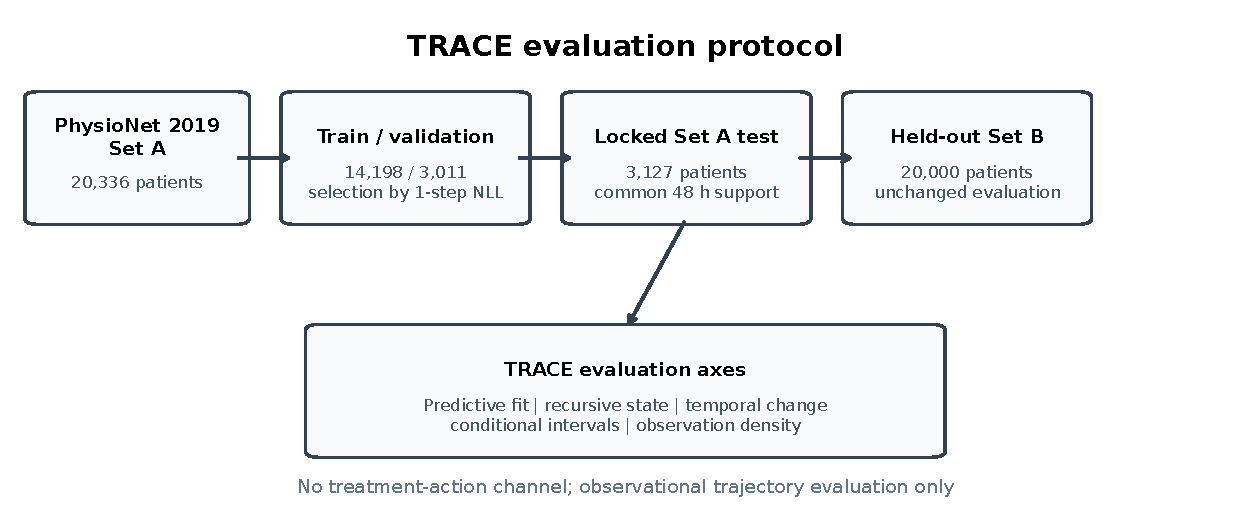
\includegraphics[width=\textwidth]{figures/pipeline.pdf}
\caption{TRACE evaluation protocol. Models are selected on Set A training/validation data, evaluated on a locked Set A test cohort across predictive fit, recursive fidelity, temporal dynamics, conditional interval reliability, and observation density, then applied unchanged to held-out Set B.}
\label{fig:framework}
\end{figure}

% =========================================================
\section{Results}
% =========================================================

\subsection{Predictive selection and recursive fidelity}

All 20 model--seed runs completed under the specified stopping rule.
Transformer achieved the lowest validation NLL
($0.8394\pm0.0020$), followed by GRU
($0.8693\pm0.0015$), Linear AR ($0.9910\pm0.0000$), and RSSM
($57.0183\pm2.3563$). Transformer also achieved the lowest internal
one-step nMacroMAE (0.4076; Table~\ref{tab:onestep}), followed closely
by Linear AR (0.4112), whereas GRU and RSSM had higher one-step errors.
The markedly poorer RSSM NLL reflected strong under-dispersion in
commonly observed variables and was consistent across the five seeds.
The five independent RSSM runs produced distinct checkpoint hashes and
validation NLL values of 58.536944, 57.891570, 52.890418, 57.341452,
and 58.431223 (mean $57.018321$, sample SD $2.3563$). All runs selected
epoch 1 as their best validation checkpoint and terminated after epoch
21 under the predefined patience-20 early-stopping rule. The
reproducibility audit confirmed that validation used the same
observed-target Gaussian NLL as the other neural architectures and did
not include the KL regularization term used during RSSM training.
Accordingly, the poor probabilistic fit is reproducible for this fixed
RSSM configuration and training protocol, rather than attributable to
an identified validation-metric inconsistency; it does not establish a
general defect of RSSM architectures.

\begin{table}[ht]
\centering
\caption{One-step predictive performance. Validation NLL defines the
conventional model-selection criterion. Set B values are interpreted
in Section~\ref{sec:setb_results}.}
\label{tab:onestep}
\small
\resizebox{\textwidth}{!}{%
\begin{tabular}{lccc}
\toprule
Model & Internal validation NLL & Internal 1-step nMacroMAE & Set B 1-step NLL \\
\midrule
Linear AR & $0.9910\pm0.0000$ & 0.4112 & $1.7557\pm0.0000$ \\
GRU & $0.8693\pm0.0015$ & 0.4484 & $1.6092\pm0.0437$ \\
Transformer & $\mathbf{0.8394\pm0.0020}$ & \textbf{0.4076} & $\mathbf{1.5749\pm0.0935}$ \\
RSSM & $57.0183\pm2.3563$ & 0.6230 & $14.6212\pm1.1809$ \\
\bottomrule
\end{tabular}
}
\end{table}

Thus, before recursive evaluation, conventional predictive selection
clearly favored Transformer. Recursive state fidelity increasingly
departed from this one-step ordering as rollout horizon increased
(Figure~\ref{fig:rollout}a).

At 48 h, RSSM ranked first numerically with nMacroMAE
0.765 [0.740, 0.790], followed by Transformer at
0.769 [0.727, 0.818] and GRU at 0.786 [0.738, 0.835].
However, the paired Transformer--RSSM difference was only
0.0036 (95\% CI $[-0.0424,0.0622]$), so the apparent change in
the top-ranked model was not statistically resolved. The predefined
criterion for a supported primary model-selection reversal was therefore
not met.

Linear AR exhibited a different failure mode. Its nMacroMAE increased
from 0.560 [0.543, 0.577] at 4 h to 4.582 [4.327, 4.818] at 48 h,
with a 48-h Linear AR--RSSM difference of
3.8165 [3.5683, 4.0565]. Recursive degradation was therefore substantial
for Linear AR, whereas the long-horizon difference between Transformer
and RSSM remained statistically unresolved.

\begin{figure}[ht]
\centering
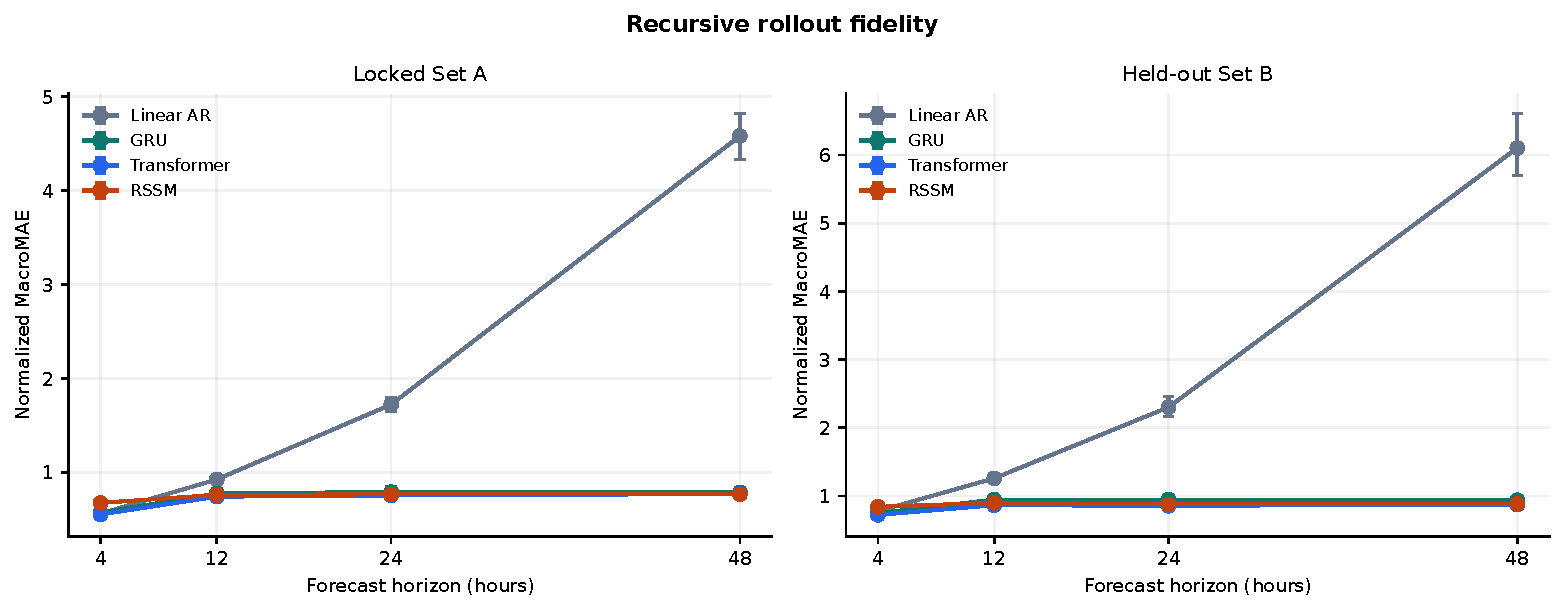
\includegraphics[width=\textwidth]{figures/figure2_rollout_fidelity.pdf}
\caption{Recursive rollout fidelity across horizons. Lower normalized
MacroMAE indicates better state fidelity. Error bars show hierarchical
paired bootstrap 95\% confidence intervals.}
\label{fig:rollout}
\end{figure}


\subsection{Temporal dynamics, reliability, and observation density}

Recursive state error does not determine whether a model reproduces
how physiological states change over time. At 48 h internally,
DynamicMAE ranked RSSM first (0.279), Transformer second (0.283),
GRU third (0.288), and Linear AR fourth (0.348). In contrast to the
48-h state-fidelity comparison, the Transformer--RSSM DynamicMAE
difference excluded zero (0.00372, 95\% CI [0.00093, 0.00650]),
supporting lower temporal-change error for the evaluated RSSM
configuration.

This advantage did not imply better preservation of temporal variability.
Predicted-to-observed change-variance ratios were 0.301 for GRU,
0.238 for Transformer, and 0.121 for RSSM, indicating contraction of
temporal variability by all three neural models, with the strongest
contraction for RSSM. Linear AR showed the opposite behavior, with
severe variance inflation (ratio 78.738; Figure~\ref{fig:dynamics}).
Thus, RSSM combined lower first-difference error with substantially
smoother-than-observed trajectories, showing that DynamicMAE and
variability preservation provide complementary evidence.

\begin{figure}[!ht]
\centering
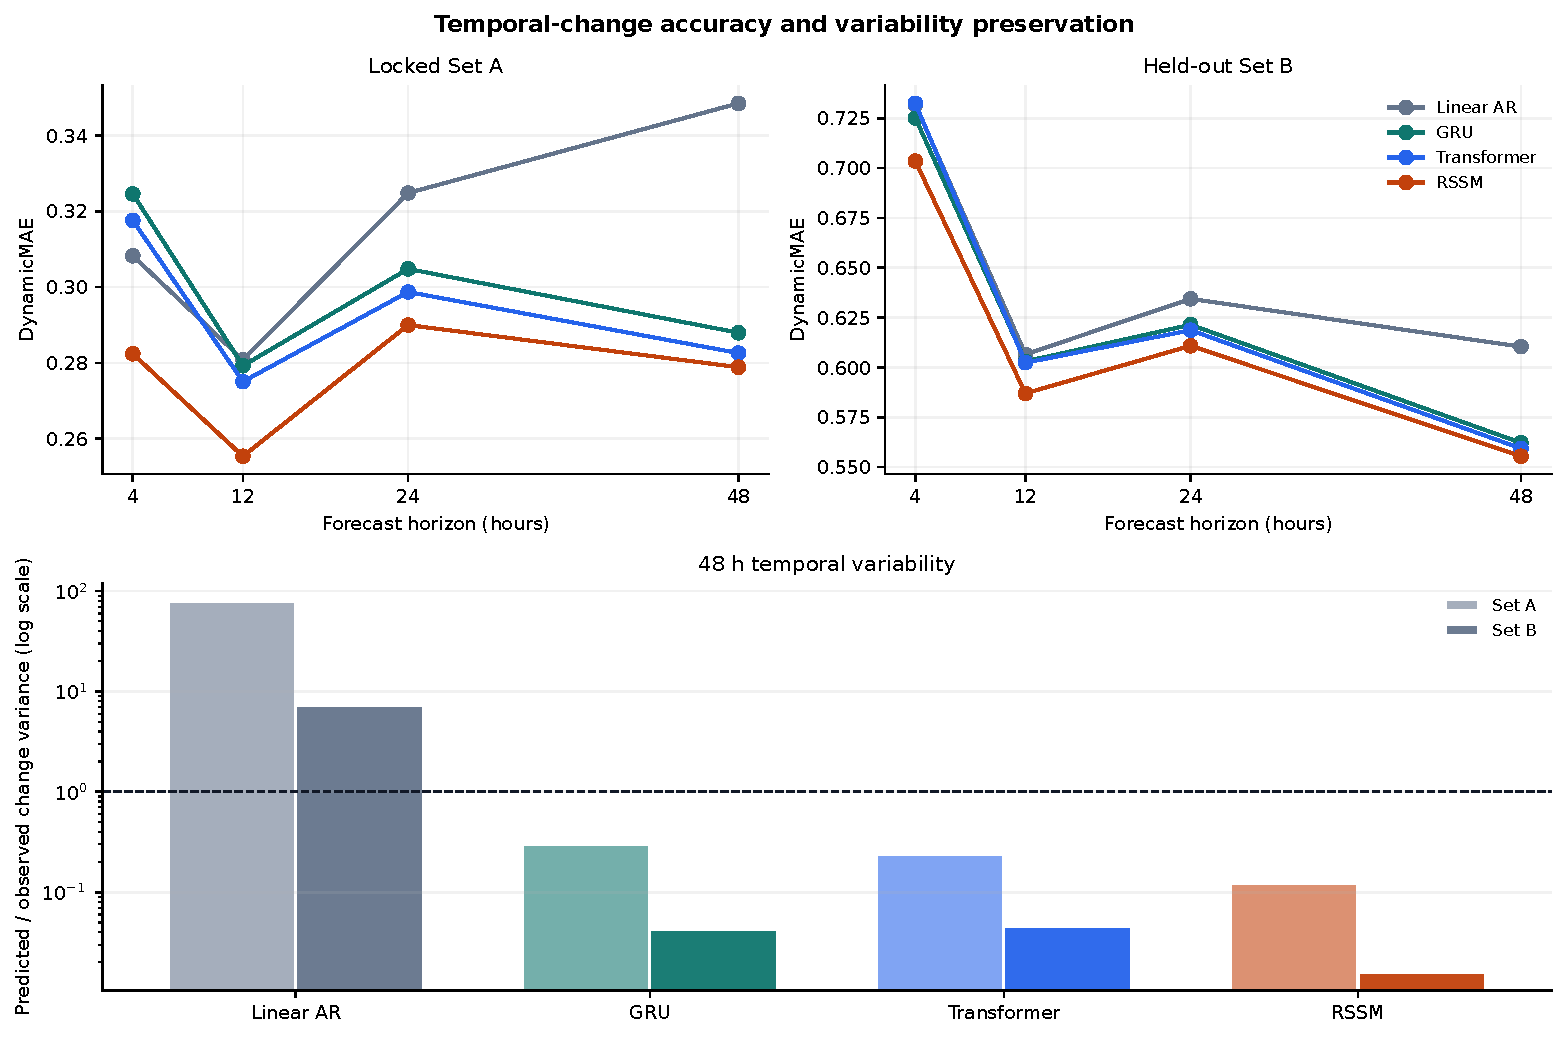
\includegraphics[width=\textwidth]{figures/figure3_temporal_dynamics.pdf}
\caption{Temporal-change accuracy and variability preservation.
Lower DynamicMAE indicates smaller temporal-change error. The lower
panel shows the 48-h predicted-to-observed change-variance ratio;
unity denotes matched temporal variability.}
\label{fig:dynamics}
\end{figure}

Transformer provided the most reliable internal conditional predictive
intervals under the evaluated deterministic mean-rollout procedure.
At 48 h, empirical coverage was 0.472, 0.769, and 0.911 for nominal
50\%, 80\%, and 95\% intervals, respectively, yielding an absolute
95\%-coverage error of 0.059. The resulting reliability ordering was
Transformer $>$ GRU $>$ RSSM $>$ Linear AR.

Although Transformer was closest to nominal coverage, its empirical
coverage remained below nominal at all three reported levels; therefore,
``most reliable'' should not be interpreted as perfectly calibrated.
Linear AR was markedly under-covered, with empirical coverage of only
0.254 at the nominal 95\% level, while RSSM was also more under-covered
than Transformer (Figure~\ref{fig:reliability}). These intervals remain
conditional on deterministic mean rollout and do not represent fully
propagated stochastic trajectory uncertainty.

\begin{figure}[!ht]
\centering
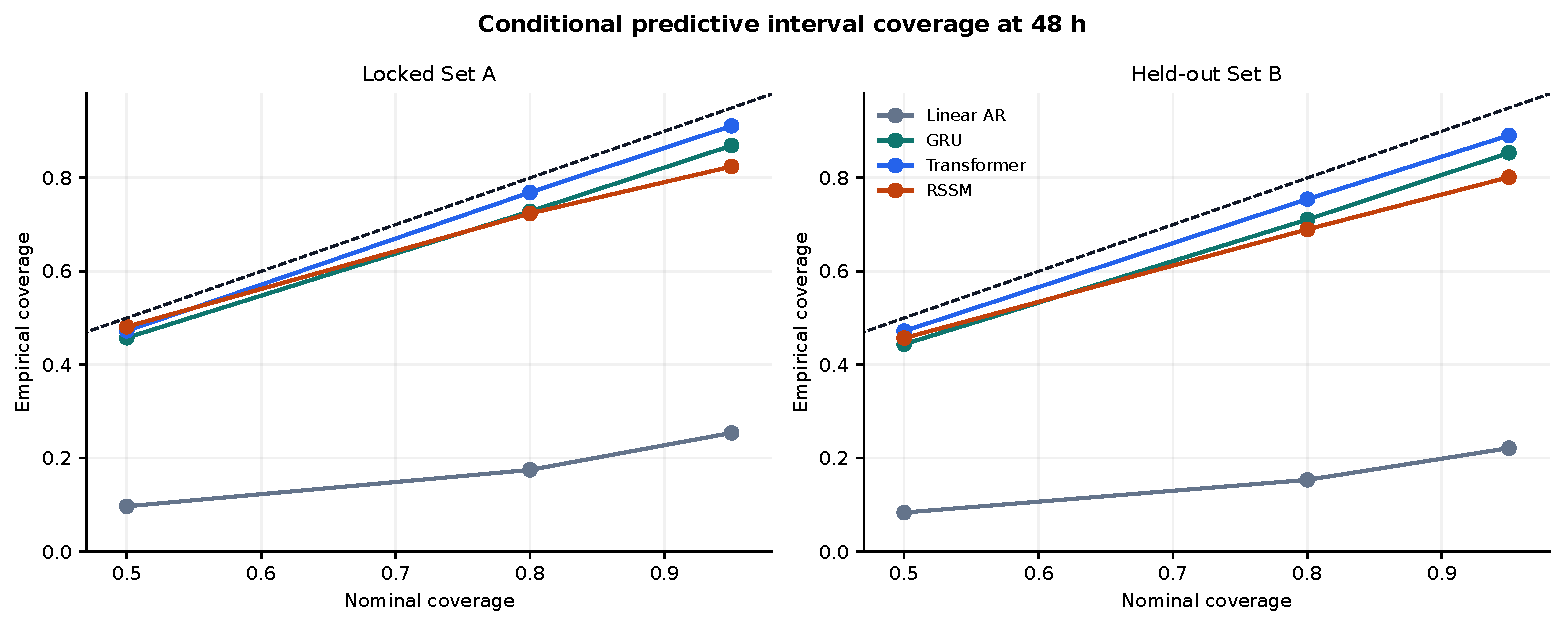
\includegraphics[width=\textwidth]{figures/figure4_interval_coverage.pdf}
\caption{Nominal versus empirical coverage of conditional predictive
intervals at 48 h. The diagonal denotes nominal coverage.}
\label{fig:reliability}
\end{figure}

Observation density provided a further source of heterogeneity in model
preference (Figure~\ref{fig:density}a). GRU was supported over
Transformer and RSSM for the predefined core-dense variables, whereas
RSSM was supported over both neural competitors in the 80--95\%
missingness stratum. In the other $\leq80\%$ and $>95\%$ strata,
numerical leaders were not statistically distinguishable from their
closest competitors. All three deep models outperformed Linear AR in
every observation-density stratum.

These results show that a global model ranking does not necessarily
represent performance within a particular measurement regime: the model
supported for frequently observed physiological variables differed from
that supported for substantially sparser variables.

\begin{figure}[!ht]
\centering
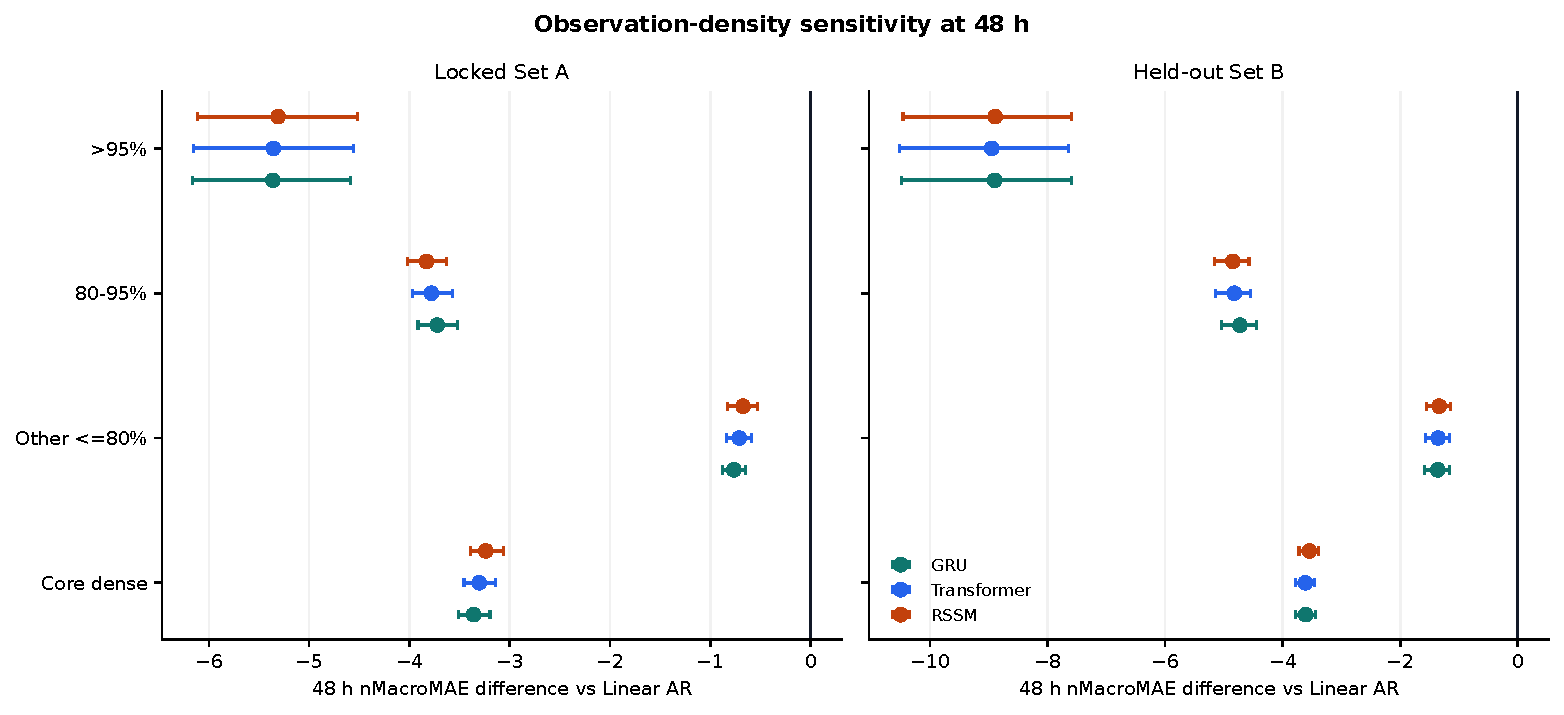
\includegraphics[width=\textwidth]{figures/figure5_observation_density.pdf}
\caption{Observation-density sensitivity at 48 h. Values are paired
normalized-MAE differences relative to Linear AR; negative values favor
the deep model. Error bars show paired bootstrap 95\% confidence
intervals.}
\label{fig:density}
\end{figure}


\subsection{Internal synthesis and held-out Set B}
\label{sec:setb_results}

Taken together, the internal evaluation yielded criterion-dependent
evidence rather than a criterion-independent model winner. Transformer
was selected by validation NLL, achieved the lowest internal one-step
error, and provided the most reliable conditional intervals. Transformer
and RSSM remained statistically unresolved for 48-h recursive state
fidelity. RSSM achieved lower 48-h DynamicMAE, but this advantage
coexisted with the strongest neural temporal-variance contraction.
Observation-density stratification further favored GRU in the core-dense
group and RSSM in the 80--95\% missingness group.

The internal evidence therefore did not support replacing Transformer
globally with RSSM as rollout horizon increased. Rather, the preferred
model depended on the property used to define adequacy.

Set B was then used to test whether this multi-axis pattern transported
to a second hospital system, without retraining, recalibration, or
revision of the evaluation rules. It preserved the overall pattern
without reproducing an identical numerical architecture ranking.

Transformer remained first by one-step NLL
($1.5749\pm0.0935$). At 48 h, Transformer ranked first numerically
for recursive state fidelity
(0.8732 [0.8357, 0.9129]), followed by RSSM
(0.8850 [0.8603, 0.9095]). Their paired difference again included zero
($-0.01181$, 95\% CI $[-0.04302,0.02068]$), reproducing the internal
finding that the two models were not statistically resolved on
long-horizon state fidelity. Linear AR again degraded markedly, reaching
6.1021 [5.6982, 6.6039] at 48 h.

The temporal-change result also transported. RSSM retained the
48-h DynamicMAE advantage, with
0.5452 [0.5012, 0.5963] versus
0.5489 [0.5049, 0.5999] for Transformer; the paired difference was
0.00367 [0.00211, 0.00532]. Neural temporal-variance contraction became
even stronger on Set B, with ratios of 0.0425 for GRU, 0.0458 for
Transformer, and 0.0160 for RSSM, whereas Linear AR remained
inflationary (7.2376).

Conditional interval reliability also preserved the internal ordering.
Transformer again had the lowest absolute 95\%-coverage error (0.0705),
followed by GRU (0.1034), RSSM (0.1633), and Linear AR (0.7286).
Observation-density dependence likewise persisted: RSSM retained a
supported advantage in the 80--95\% missingness stratum, whereas the
numerical leaders in the core-dense and sparsest strata were not
consistently distinguishable.

\begin{table}[ht]
\centering
\caption{Decision-oriented synthesis of the reported results. ``Unresolved'' refers to the reported paired confidence interval, not equivalence of models.}
\label{tab:decision_summary}
\small
\begin{tabularx}{\textwidth}{p{3.0cm}p{3.5cm}X}
\toprule
Evaluation priority & Locked Set A evidence & Held-out Set B evidence \\
\midrule
One-step predictive fit & Transformer lowest validation NLL and one-step nMacroMAE & Transformer lowest one-step NLL \\
48-h recursive state fidelity & RSSM numerically first; Transformer--RSSM contrast unresolved & Transformer numerically first; same contrast unresolved \\
48-h temporal-change error & RSSM lower DynamicMAE than Transformer; paired CI excludes zero & RSSM lower DynamicMAE; paired CI excludes zero \\
Temporal-change variability & RSSM most contracted among neural models; Linear AR inflated & Neural contraction stronger; Linear AR inflated \\
95\% conditional-interval coverage & Transformer closest to nominal but still under-covering & Transformer smallest absolute coverage error, still under-covering \\
Observation-density sensitivity & GRU favored in core-dense; RSSM in 80--95\% missingness & RSSM advantage persists in 80--95\% missingness; core-dense leaders not consistently resolved \\
\bottomrule
\end{tabularx}
\end{table}

Thus, Set B did not reproduce every internal numerical ranking. It
reproduced the central TRACE result: predictive fit, recursive state
fidelity, temporal-change accuracy, temporal variability, conditional
uncertainty reliability, and observation density provide distinct
model-selection evidence rather than a single interchangeable ranking.

% =========================================================
\section{Discussion}
% =========================================================

\subsection{Model selection depends on the required property}

TRACE shows that changing the property required of a longitudinal model changes the evidence used to select it. Transformer was consistently favored by conventional predictive criteria and conditional interval reliability. RSSM had lower 48-h temporal-change error, but Transformer and RSSM remained statistically unresolved for 48-h state fidelity in both hospital systems. The distinction between a numerical rank change and a supported selection difference is therefore central: point estimates alone would have suggested different state-fidelity leaders internally and externally, whereas paired uncertainty does not support that conclusion.

This is more restrictive than simply recommending additional metrics. Predictive likelihood, recursive state error, temporal-change error, temporal variability, uncertainty reliability, and observation-density robustness test different properties. Their disagreement is not noise to average away; it identifies which evidence is required for a given intended use. TRACE should therefore be read as a fit-for-purpose evaluation framework rather than a leaderboard.

The RSSM findings further illustrate why an isolated improvement in
temporal-change error should not be equated with overall trajectory
quality. A configuration may rank favorably on one evaluation axis
while exhibiting substantial deficiencies in predictive likelihood,
temporal variability, and uncertainty reliability. This disagreement
is precisely the model-selection evidence that TRACE is designed to
expose rather than conceal through a single aggregate score. TRACE is
therefore an evaluation framework for matching evidence to an intended
use, not a new forecasting architecture or an architecture leaderboard.

\subsection{Interpreting the fixed RSSM configuration}

The RSSM findings require particular caution. Its validation NLL ($57.0183\pm2.3563$) was far worse than that of Transformer ($0.8394\pm0.0020$), and the selected checkpoint occurred at epoch 1 in all five RSSM runs. Thus, the observed advantage in 48-h DynamicMAE cannot be interpreted as evidence that RSSM architectures generally outperform Transformers on clinical dynamics. It is a result for this fixed configuration under validation-NLL checkpoint selection. The very early checkpoint selection and poor probabilistic fit raise a plausible model-configuration or optimization concern; the present experiments do not isolate which mechanism caused it. Nevertheless, the contrast remains informative for the methodological question: a candidate with poor likelihood can achieve lower error on one temporal-change statistic while simultaneously producing pronounced temporal variance contraction and poor conditional interval coverage.

An architecture-level claim would require an additional, prespecified RSSM sensitivity study, including alternative KL weights, variance parameterizations, training schedules, and checkpoint diagnostics, evaluated without consulting the locked test or Set B for model selection. Such experiments have not been performed in the reported protocol and are not implied by the existing results.

\subsection{Different axes reveal different failure modes}

RSSM illustrates why temporal-change error cannot stand alone. Its lower 48-h DynamicMAE coexisted with the strongest temporal variance contraction among neural models, internally and on Set B. A model can therefore reduce average first-difference error while producing trajectories that are too smooth. Transformer also contracted variability, but less strongly, while providing conditional intervals closer to nominal coverage. Linear AR showed the opposite failure mode: relatively competitive short-horizon error followed by severe long-horizon state error and variance inflation.

The uncertainty result must also be interpreted within the implemented rollout. Predictive means were recursively reinserted and intervals were computed conditionally along that mean path. Coverage therefore evaluates the uncertainty actually reported by these models under deterministic mean rollout, not a full probability distribution over stochastic future trajectories. A stronger uncertainty-aware simulator would require explicit propagation and evaluation of trajectory-level uncertainty.

Observation density exposed another source of heterogeneity. Internally, GRU was supported for core-dense variables and RSSM for the 80--95\% missingness group; the latter advantage persisted on Set B. Because measurement frequency is clinically triggered and correlated with variable type, the present analysis does not establish that sparsity itself causes these ranking changes. It shows that a global average can hide model behavior in the observation regime relevant to deployment.

\subsection{Transportability and implications for clinical world models}

Set B is a meaningful hospital-system stress test but not broad external validation. It shares the PhysioNet Challenge variable definitions and acquisition context with Set A. What transported was the structure of the evidence: Transformer remained strongest by predictive fit and conditional interval reliability, RSSM retained lower temporal-change error, Transformer and RSSM remained unresolved for 48-h state fidelity, density dependence persisted, neural models contracted variability, and Linear AR degraded under long rollout. Replication on unrelated datasets such as MIMIC-IV or eICU would provide a stronger generalization test.

These findings are relevant as clinical modeling moves toward longitudinal simulators, medical world models, and digital twins. A short-range predictor can reasonably be judged mainly by predictive accuracy and uncertainty reliability. A model described as a simulator additionally requires evidence of recursive stability, temporal-change behavior, and variability preservation; intervention-oriented or counterfactual claims require stronger evidence still. The present models are observational trajectory models, not validated causal models of treatment response, and none should be interpreted as ready for bedside simulation or treatment planning.

\subsection{Limitations}

Several limitations constrain interpretation. First, each forecast is
compared with one realized future, although multiple physiological
futures may be plausible; trajectory distributions, cross-variable
dependence, clinically meaningful events, and expert assessment were
not evaluated. The reported intervals are conditional on deterministic
mean feedback and do not propagate uncertainty through stochastic
future paths. Second, EHR measurements are irregular and clinically
triggered, so observed trajectories conflate latent physiology with
observation policy. Third, only four fixed model configurations were
compared, without architecture-specific hyperparameter optimization.
The fixed RSSM was especially limited: every seed selected epoch 1, its
probabilistic fit was poor, and its lower 48-h DynamicMAE coexisted with
the strongest neural temporal-variance contraction. This is
configuration-specific evidence of lower first-difference error; it
does not demonstrate general RSSM superiority, more realistic
physiological dynamics, better probabilistic trajectory generation, or
improved causal or counterfactual simulation. No additional RSSM
sensitivity experiment was performed. Fourth, bootstrap inference
addresses patient clustering and seed variability but not uncertainty
from preprocessing choices, metric design, or architecture
specification. Finally, Set B is a hospital-system comparison within a
single benchmark and shared acquisition context, not validation on an
independent dataset; transportability to unrelated health systems
remains unknown.

Future work should conduct prespecified RSSM optimization and
training-stability analyses before making claims about the model family,
and test alternative state-space configurations, direct and hybrid
direct--recursive strategies such as DRIFT \cite{liu2026drift}, emerging
clinical world-model architectures, stochastic trajectory-level
uncertainty, and independent critical-care datasets such as MIMIC-IV
and eICU.

% =========================================================
\section{Conclusion}
% =========================================================

TRACE evaluated whether conventional one-step model selection remains valid when clinical trajectory models are judged for recursive longitudinal use. It did not identify a criterion-independent winner. Transformer led predictive fit and conditional interval reliability; RSSM had lower 48-h temporal-change error but stronger temporal smoothing; Transformer and RSSM were unresolved for 48-h state fidelity; observation density altered relative performance; and Linear AR became unstable under long rollout. The axis-dependent pattern persisted across the two hospital systems, although numerical rankings did not fully reproduce. Model evaluation should therefore be specified in relation to intended use before stronger claims about longitudinal simulation, medical world models, or digital twins are made.

\section*{Data availability}
The PhysioNet/Computing in Cardiology Challenge 2019 data are available
from PhysioNet under the applicable data-use terms (version 1.0.0; DOI
10.13026/v64v-d857) \cite{reyna2020sepsis}. This study does not
redistribute source records, patient-ID split assignments, or
patient-level sufficient statistics. The reproducibility package
provides acquisition instructions, deterministic split reconstruction
with seed 4317, expected cohort counts, and a canonical split hash.

\section*{Code availability}
A versioned scientific release candidate containing source code, frozen
configurations, validation-selected checkpoints, aggregate result
tables, bootstrap replicate arrays, automated tests, figure-generation
code, and a SHA-256 artifact manifest was verified locally against Git
commit \texttt{fe5110d} (full hash recorded in the artifact manifest). All 59
reconciled manuscript values matched their canonical artifacts, and the
102-test synthetic/unit regression suite passed, including 17 targeted
methods-audit tests. At the time this manuscript was finalized, the
release had not yet been published at a verified public URL; therefore,
no public repository or archive link is claimed here. Public access
details will be added only after the redistribution-cleared package and
immutable release tag have been independently verified online.

\section*{Reproducibility and supplementary material}
The supplementary reproducibility package documents the software
environment, experiment seeds, checkpoint and artifact hashes,
evaluation and hierarchical bootstrap procedures, numerical
reconciliation, figure generation, automated tests, and known
limitations. Patient-level resources remain excluded pending
redistribution and privacy review and can be reconstructed by authorized
researchers from the original PhysioNet records using the frozen
pipeline. The Set B evaluation retains its documented E2 potential-
unblinding qualification: an early preflight reached data loading but
stopped before inference or exposure of predictions, metrics, or
rankings. External density reporting was subsequently corrected from
immutable sufficient statistics to align point estimates and intervals
to the same frozen estimand; no model inference was rerun.

\section*{Ethics statement}
This work is a secondary analysis of publicly available, de-identified PhysioNet Challenge data. The authors had no direct interaction with participants and did not attempt re-identification.

\section*{CRediT authorship contribution statement}
\textbf{Nesma Settouti:} Conceptualization, Methodology, Software, Validation, Formal analysis, Investigation, Data curation, Writing -- original draft, Writing -- review \& editing, Visualization, Project administration.\\
\textbf{Souaad Hamza-Cherif:} Conceptualization, Formal analysis, Writing -- review \& editing.\\
\textbf{Mohammed El Amine Bechar:} Formal analysis, Writing -- review \& editing.

\section*{Funding}
This research did not receive any specific grant from funding agencies in the public, commercial, or not-for-profit sectors.

\section*{Declaration of competing interest}
The authors declare that they have no known competing financial interests or personal relationships that could have appeared to influence the work reported in this paper.

\section*{Declaration of generative AI and AI-assisted technologies in the manuscript preparation process}
During the preparation of this work, the authors used OpenAI ChatGPT to support organization, language refinement, and clarity. The authors reviewed and edited the output as needed and take full responsibility for the published content.

\bibliographystyle{elsarticle-num}
\bibliography{trace_jbi_references_v4}

\end{document}
